\subsection{Замечания относительно пакета glpk}

Существенный объём времени был потрачен на выяснение причин, по которым пакет glpk не решал задачи, поставленные в модуле ir\_outer.m (минимизация и максимизация $\beta_0$ и $\beta_1$ покомпонентно). Выяснилось, что солвер revised\_simplex не в состоянии найти решения этих задач. Кроме того, солвер interior\_point не мог найти граничные $\beta_0$ и $\beta_1$, когда на переменные не устанавливалось ограничений снизу. После того, как было установлено дефолтное ограничение снизу (т.е 0), interior\_point со всеми задачами успешно справился. В то же время, солвер revised\_simplex в пакете scipy успешно решал те же задачи без искусственных ограничений. Эти проблемы значительно усложнили реализацию данной лабораторной работы, и их, на мой взгляд, следует обнародовать среди студентов.

\subsection{Результаты}

Ниже приведены графики, полученные в результате работы реализованной программы.

\begin{figure}[H]
	\begin{center}
		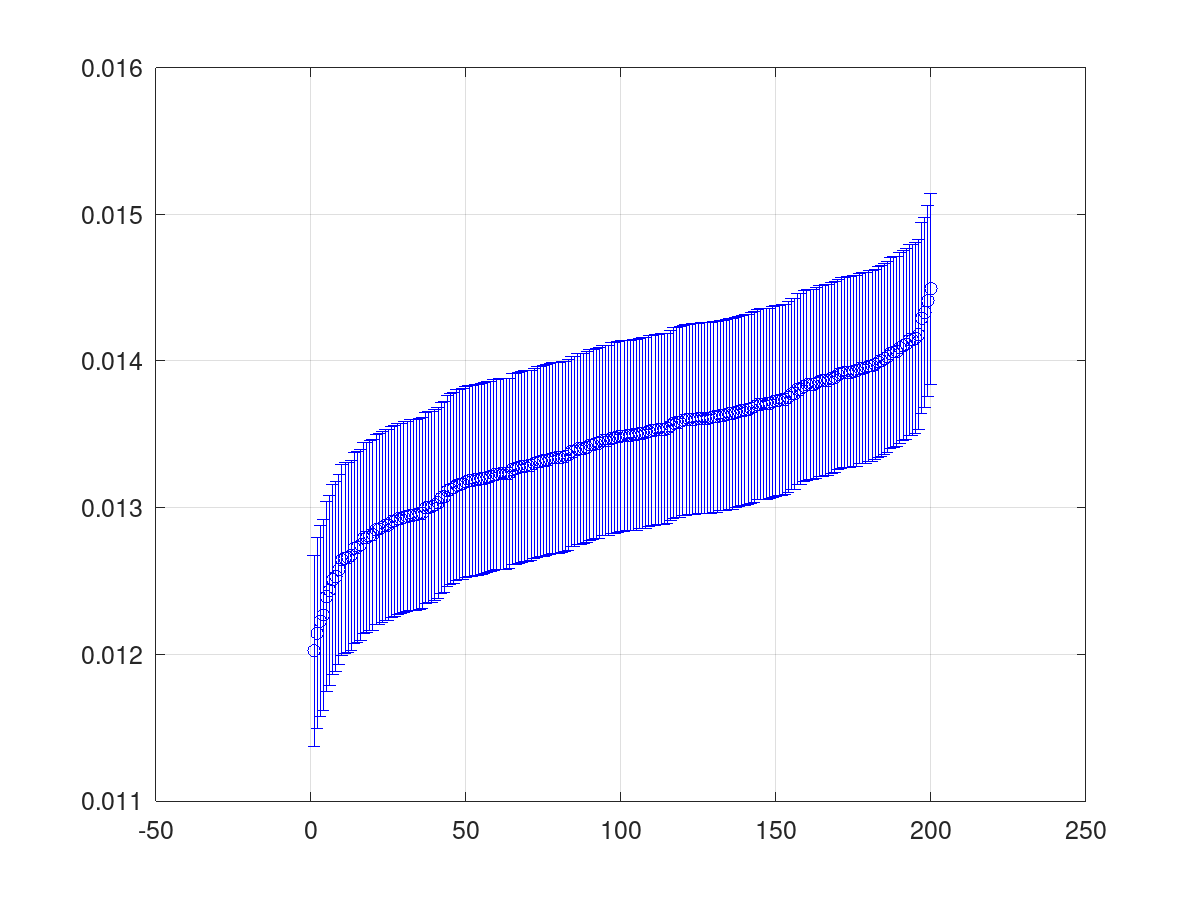
\includegraphics[scale=0.29]{interval_problem_1}
		\label{pic:model1}
		\caption{Обынтерваленные данные. Модель 1}
	\end{center}
\end{figure}

\begin{figure}[H]
	\begin{center}
		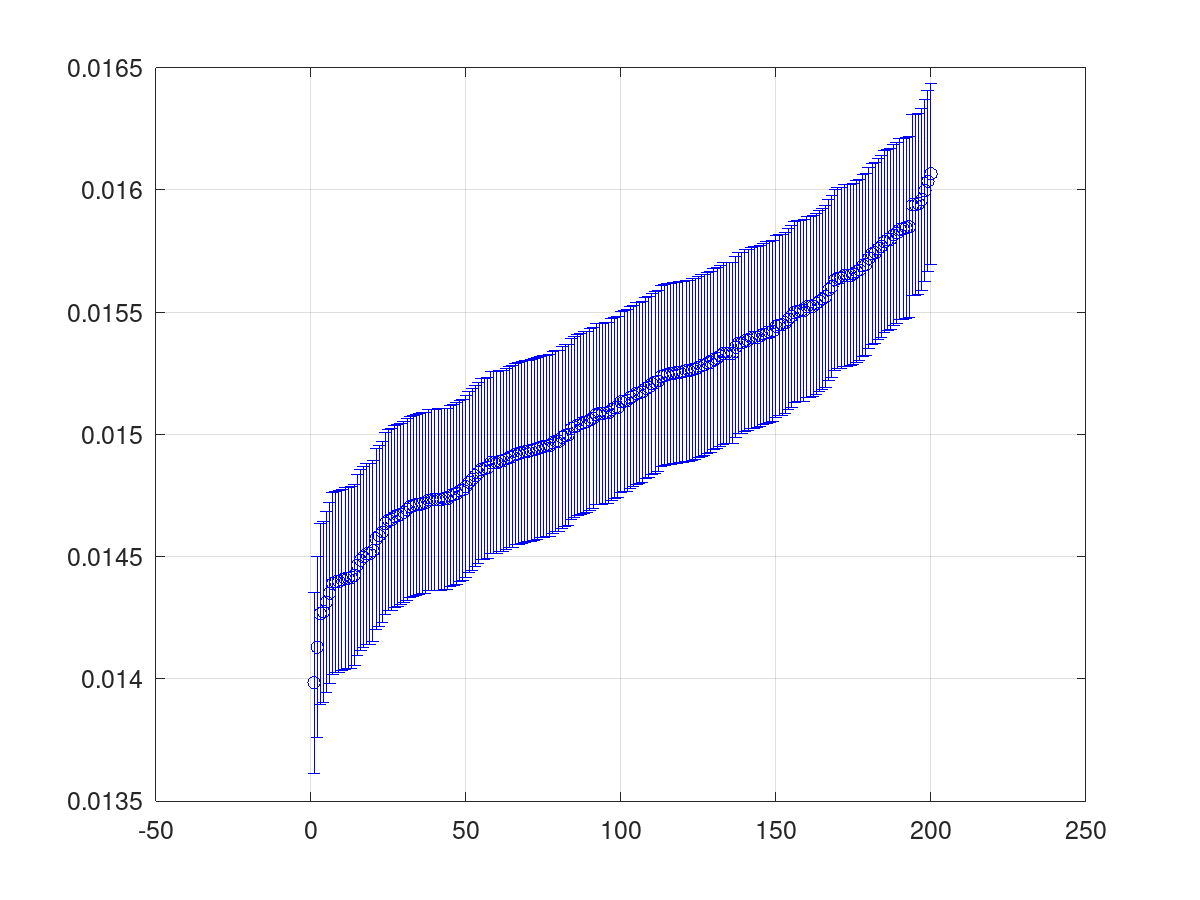
\includegraphics[scale=0.29]{interval_problem_2}
		\label{pic:model2}
		\caption{Обынтерваленные данные. Модель 2}
	\end{center}
\end{figure}

Для ускорения вычислительных процессов и более простого взаимодействия с данными, все интервалы были расширены в максимум из всех полученных весов раз: ширина интервалов составляети $\varepsilon \cdot \max_{i=\overline{1,n}(w_i)}$.

В следующей таблице приведены некоторые отличные от единицы веса:

\begin{table}[H]
	\begin{center}
		\begin{tabular}{|c|c|c|}
			\hline
			Номер интервала & Вес (модель 1) & Вес (модель 2) \\
			\hline
			1 & 6.49 & 3.70 \\
			\hline
			2 & 5.38 & 2.33 \\
			\hline
			3 & 4.63 & 1.04 \\
			\hline
			199 & 2.01 & 1.15  \\
			\hline
			200 & 2.76 & 1.37 \\
			\hline
		\end{tabular}
		\caption{Веса интервалов.}
	\end{center}
\end{table}

В обоих случай максимальный вес пришёлся на первый интервал.

\begin{figure}[H]
	\begin{center}
		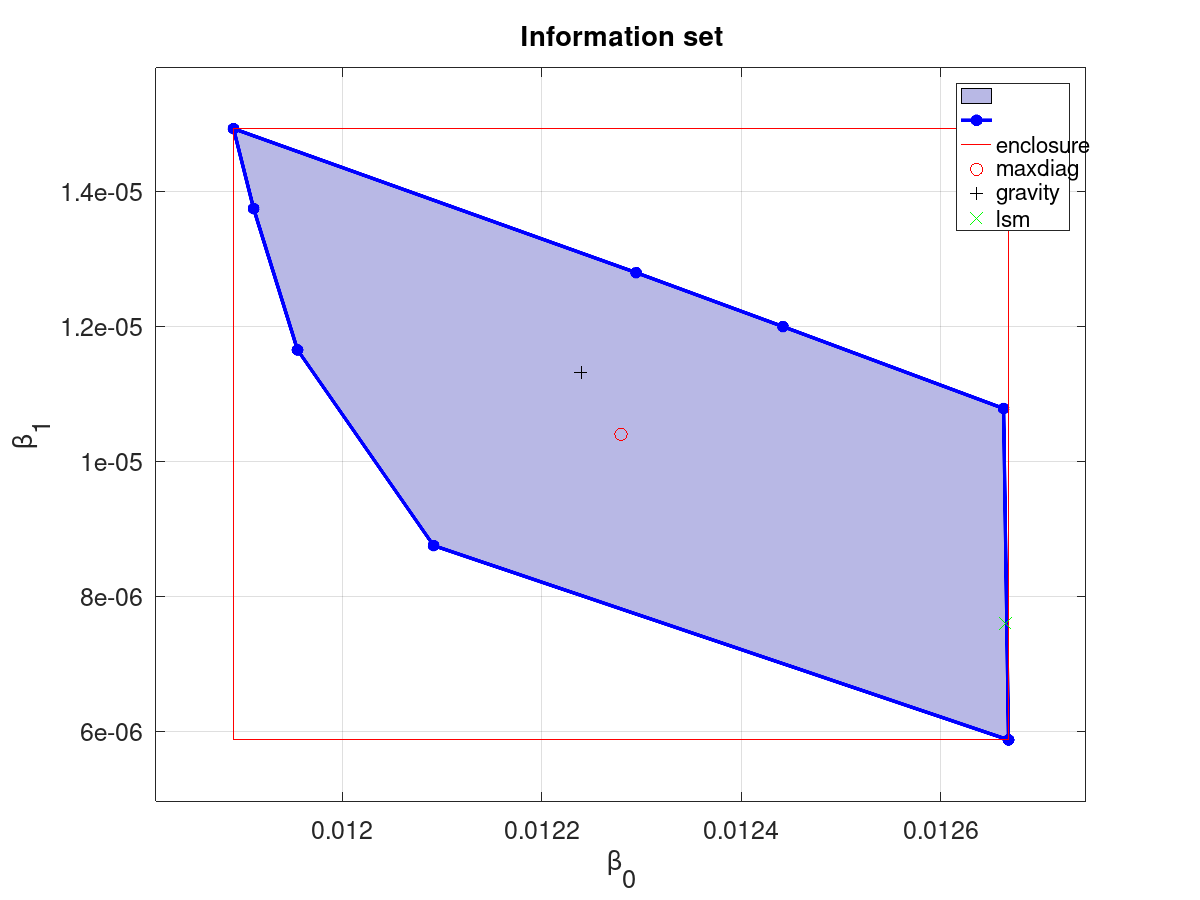
\includegraphics[scale=0.32]{info_set_full_1}
		\label{pic:infoset1}
		\caption{Информационное множество. Модель 1}
	\end{center}
\end{figure}

\begin{figure}[H]
	\begin{center}
		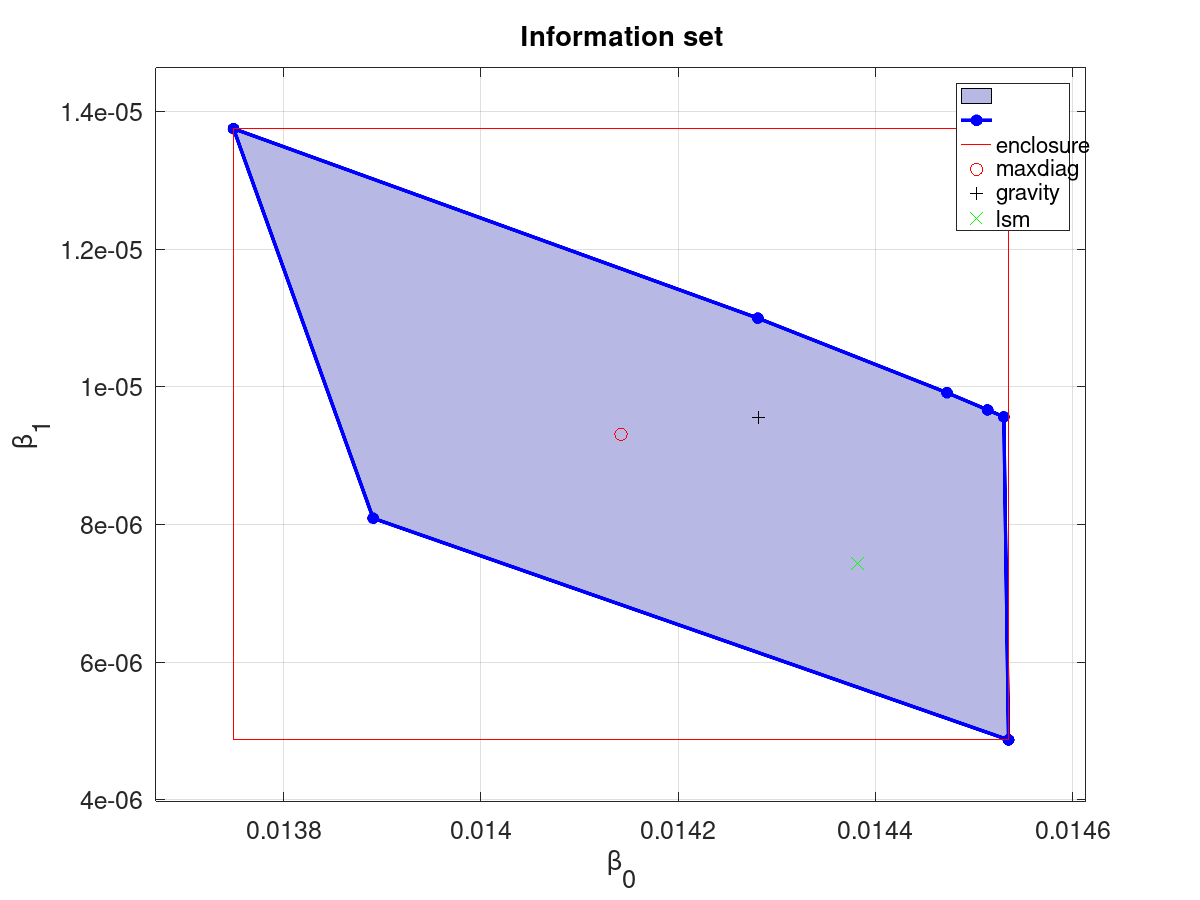
\includegraphics[scale=0.32]{info_set_full_2}
		\label{pic:infoset2}
		\caption{Информационное множество. Модель 2}
	\end{center}
\end{figure}

\begin{figure}[H]
	\begin{center}
		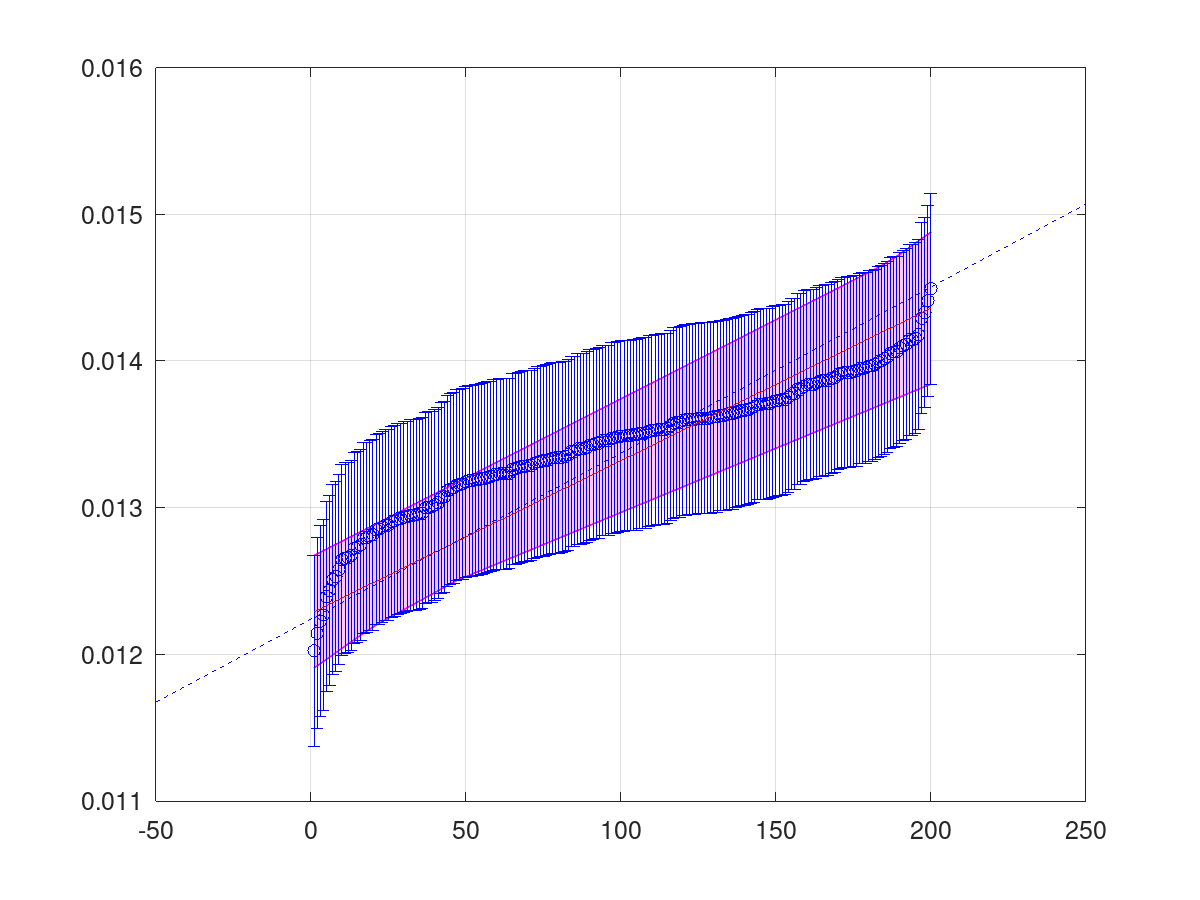
\includegraphics[scale=0.32]{joint_depth_1}
		\label{pic:joint_depth1}
		\caption{Коридор совместных зависимостей. Модель 1}
	\end{center}
\end{figure}

\begin{figure}[H]
	\begin{center}
		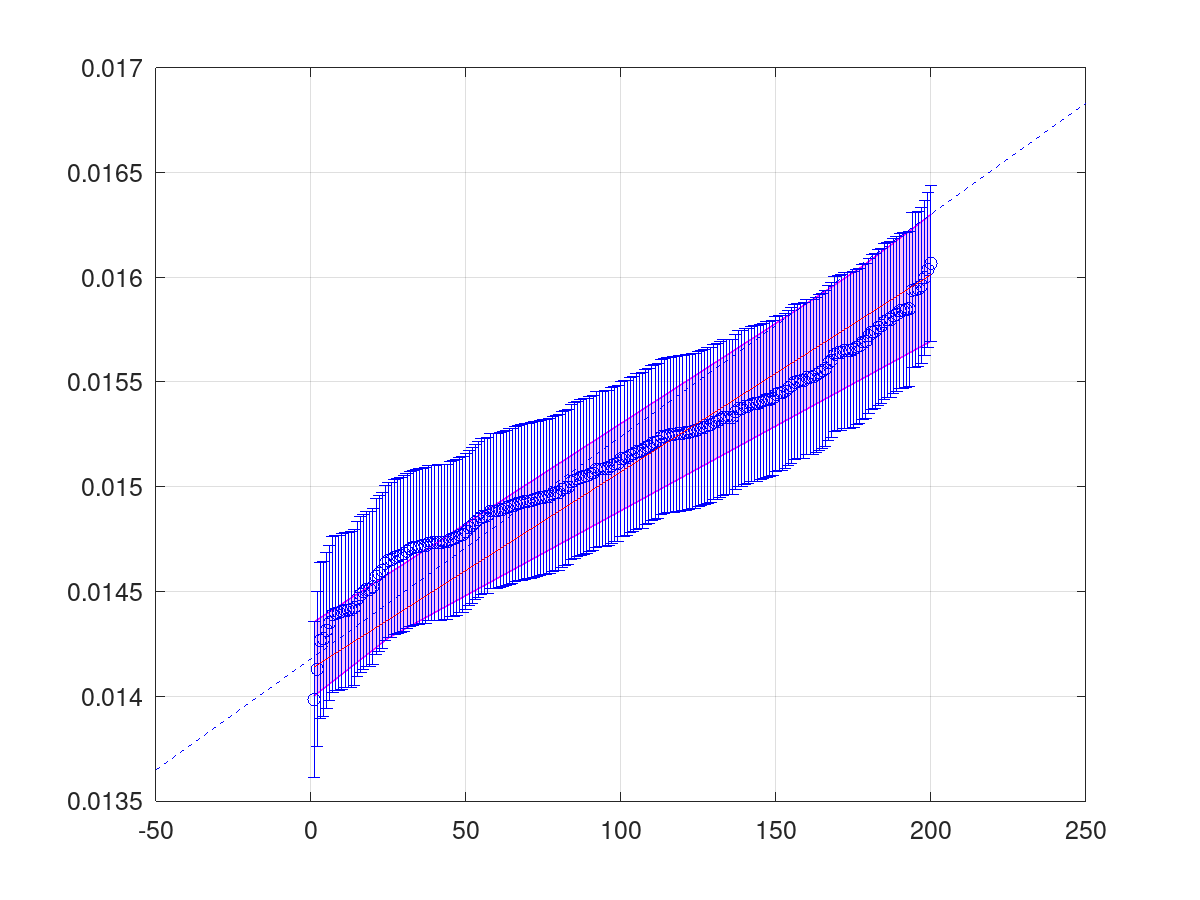
\includegraphics[scale=0.32]{joint_depth_2}
		\label{pic:joint_depth2}
		\caption{Коридор совместных зависимостей. Модель 2}
	\end{center}
\end{figure}

\begin{figure}[H]
	\begin{center}
		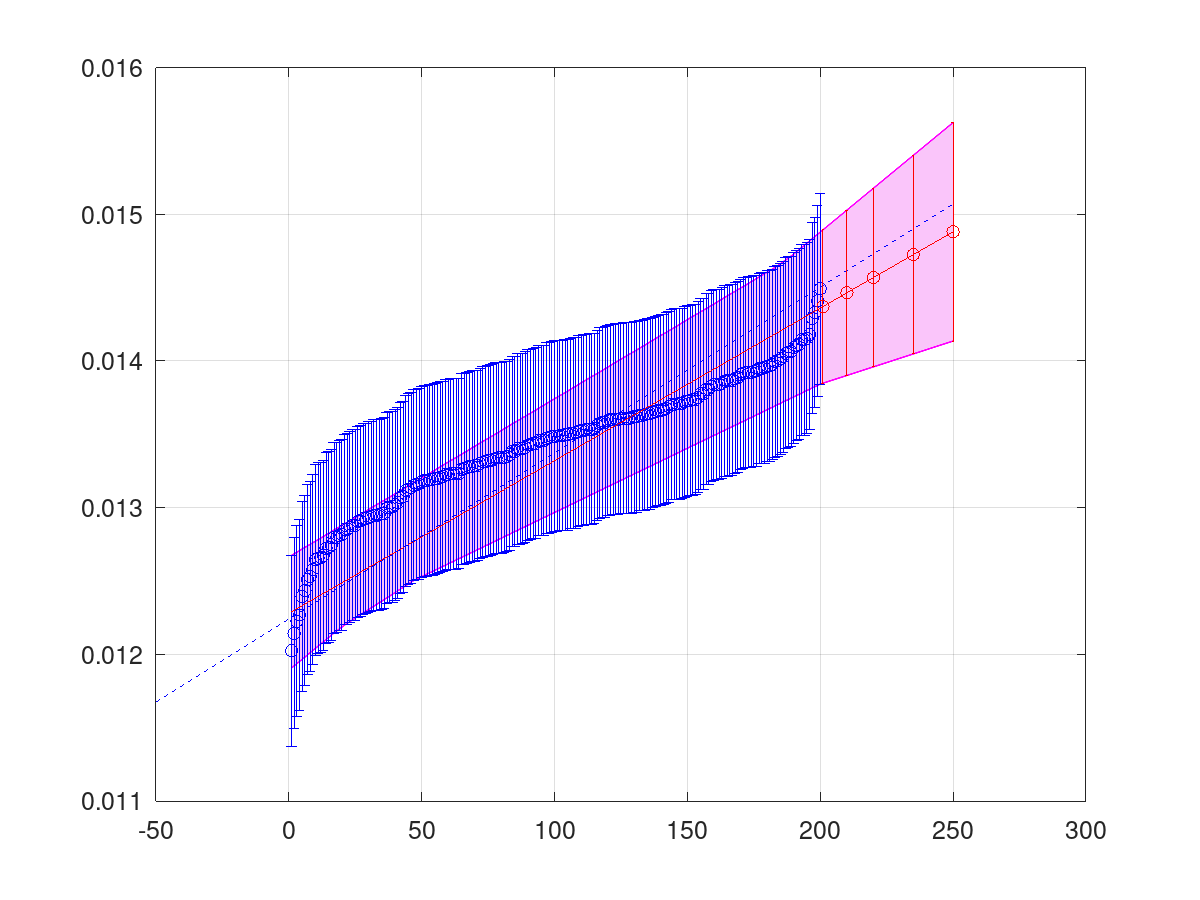
\includegraphics[scale=0.32]{prediction_1}
		\label{pic:prediction1}
		\caption{Коридор совместных зависимостей. Предсказанные значения. Модель 1}
	\end{center}
\end{figure}

\begin{figure}[H]
	\begin{center}
		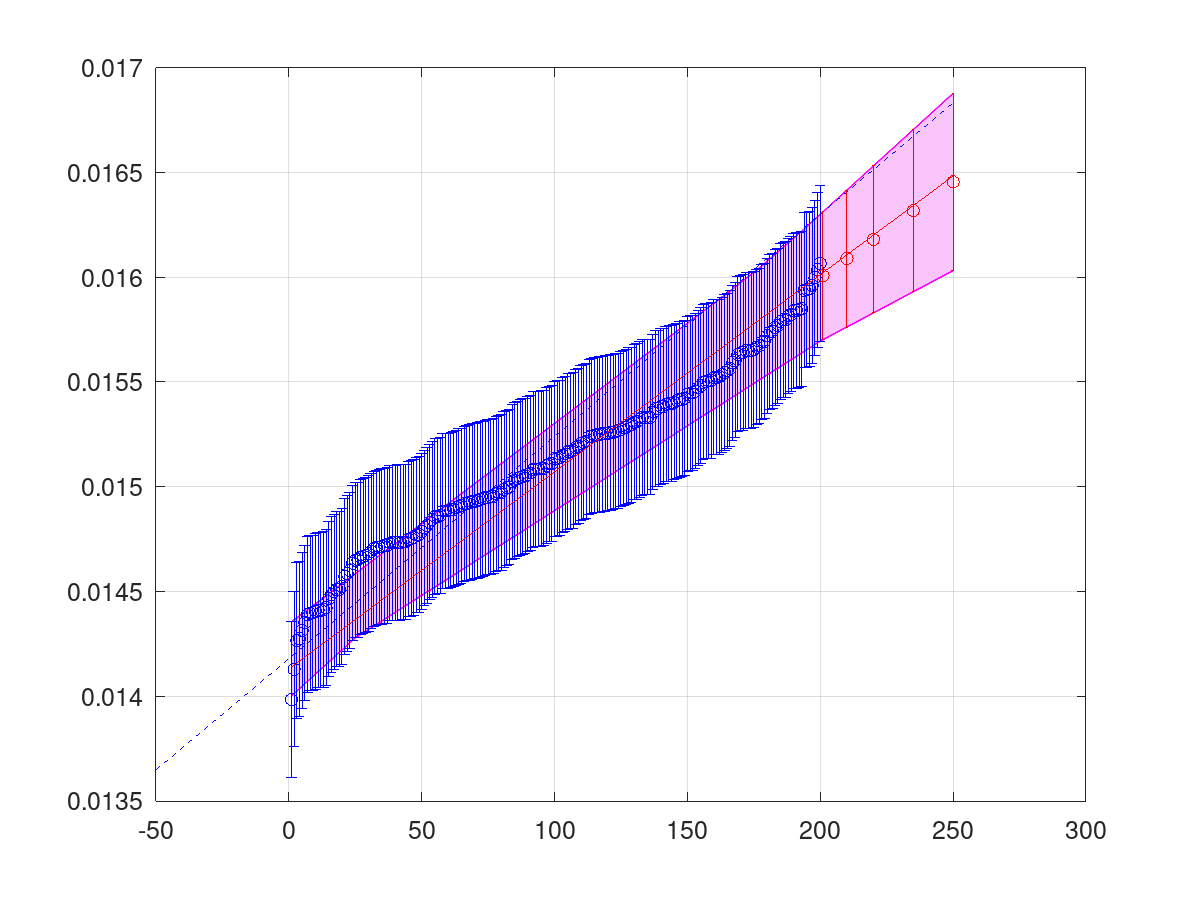
\includegraphics[scale=0.32]{prediction_2}
		\label{pic:prediction2}
		\caption{Коридор совместных зависимостей. Предсказанные значения. Модель 2}
	\end{center}
\end{figure}

Граничные точки в первой модели -- точки под номерами 1, 17, 21, 47, 182, 184, 189, 200.

Граничные точки во второй модели -- 1, 25, 162, 165, 177, 193, 200.

Максимальный коэффициент Жаккара, рассчитанный прежним методом при параметрах $\beta_0, \beta_1$, полученных как точка пересечения максимальных диагоналей (maxdiag) оказался равен 0.0615, в то время как в прошлой реализации он равен 0.037, что в 1.65 раз выше. Оптимальный коэффициент $R_{21}$ в таком случае равен 0.882, что отличается от прошлого варианта на 0.003.

\begin{figure}[H]
	\begin{center}
		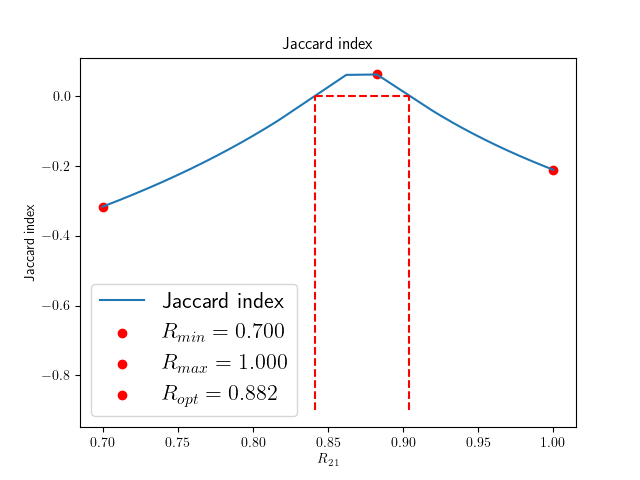
\includegraphics[scale=0.52]{jaccard}
		\label{pic:jaccard}
		\caption{Зависимость коэффициента Жаккара от множителя $R_{21}$}
	\end{center}
\end{figure}

